\documentclass[aspectratio=169]{beamer}

% =================================================================
%  Introduction to Industrial Control Systems
%  A beginner-friendly Beamer deck (fully self-contained: all
%  figures / flowcharts / plots drawn with TikZ, so it compiles anywhere).
% =================================================================

% -------------------------------------------------
% Theme and packages
% -------------------------------------------------
\usetheme{Madrid}
\usecolortheme{default}

\usepackage{amsmath}
\usepackage{amssymb}
\usepackage{bm}
\usepackage{listings}
\usepackage{tikz}
\usepackage{array}
\usepackage{booktabs}
\usepackage{tabularx}
\usepackage{ragged2e}
\usepackage{xcolor}

\usetikzlibrary{shapes.geometric, arrows.meta, positioning, calc, fit, backgrounds, patterns}

% -------------------------------------------------
% Colour palette
% -------------------------------------------------
\definecolor{cAccent}{RGB}{0,102,153}     % teal-blue accent
\definecolor{cBox}{RGB}{28,31,42}          % dark box
\definecolor{cGreen}{RGB}{34,139,34}
\definecolor{cRed}{RGB}{178,34,34}
\definecolor{cOrange}{RGB}{204,102,0}
\definecolor{cPurple}{RGB}{102,45,145}
\definecolor{cGrayBg}{RGB}{245,246,248}
\definecolor{codebg}{RGB}{248,248,244}
\definecolor{codekw}{RGB}{0,0,180}
\definecolor{codecomment}{RGB}{0,130,0}
\definecolor{codestr}{RGB}{170,55,20}

% Beamer colour tweaks (match a Madrid-style accent)
\setbeamercolor{structure}{fg=cAccent}
\setbeamertemplate{frametitle continuation}{%
	\ifnum\insertcontinuationcount>1\space(cont...)\fi
}
\setbeamertemplate{navigation symbols}{}
\setbeamertemplate{caption}[numbered]

% -------------------------------------------------
% Listings style for C code
% -------------------------------------------------
\lstdefinestyle{cstyle}{
	language=C,
	backgroundcolor=\color{codebg},
	basicstyle=\ttfamily\footnotesize,
	keywordstyle=\color{codekw}\bfseries,
	commentstyle=\color{codecomment}\itshape,
	stringstyle=\color{codestr},
	numbers=none,
	numberstyle=\tiny\color{gray},
	numbersep=8pt,
	showstringspaces=false,
	breaklines=true,
	frame=single,
	rulecolor=\color{gray!50},
	tabsize=2,
	columns=fullflexible,
	keepspaces=true,
	literate={~}{{$\sim$}}1
}
\lstset{style=cstyle}

% Listings style for IEC 61131-3 Structured Text
\lstdefinelanguage{st}{
	morekeywords={IF,THEN,ELSE,ELSIF,END_IF,VAR,END_VAR,BOOL,TIME,TON,AND,OR,NOT,IN,PT,Q,TRUE,FALSE},
	morecomment=[s]{(*}{*)},
	sensitive=true
}
\lstdefinestyle{ststyle}{
	style=cstyle,
	language=st,
	breaklines=false,
	keywordstyle=\color{codekw}\bfseries,
	commentstyle=\color{codecomment}\itshape
}

% Handy TikZ flowchart node styles
\tikzset{
	startstop/.style={rectangle, rounded corners=10pt, minimum width=2.4cm, minimum height=0.8cm, text centered, align=center, draw=black, fill=cAccent!25},
	process/.style  ={rectangle, minimum width=2.6cm, minimum height=0.8cm, text centered, align=center, text width=2.8cm, draw=black, fill=blue!8},
	io/.style       ={trapezium, trapezium left angle=70, trapezium right angle=110, minimum width=2.2cm, minimum height=0.8cm, text centered, align=center, draw=black, fill=cOrange!20},
	decision/.style ={diamond, aspect=2, minimum width=2.4cm, minimum height=0.9cm, text centered, text width=2.2cm, draw=black, fill=cGreen!18, inner sep=1pt},
	flowarrow/.style={-{Stealth[length=2.5mm]}, thick},
	% control-system block diagram styles
	blk/.style      ={rectangle, draw=black, thick, minimum width=1.9cm, minimum height=0.9cm, align=center, fill=blue!8},
	sumj/.style     ={circle, draw=black, thick, minimum size=0.55cm, inner sep=0pt},
	sig/.style      ={-{Stealth[length=2.2mm]}, thick},
}

% Ladder-logic symbols: normally-open / normally-closed contact and coil
\newcommand{\ladNO}[3]{%
	\draw[thick] ({#1-0.15},{#2-0.25}) -- ({#1-0.15},{#2+0.25});
	\draw[thick] ({#1+0.15},{#2-0.25}) -- ({#1+0.15},{#2+0.25});
	\node[above=1pt, font=\scriptsize] at (#1,{#2+0.25}) {#3};}
\newcommand{\ladNC}[3]{%
	\ladNO{#1}{#2}{#3}
	\draw[thick] ({#1-0.25},{#2-0.3}) -- ({#1+0.25},{#2+0.3});}
\newcommand{\ladCoil}[3]{%
	\draw[thick] (#1,#2) circle (0.28);
	\node[above=1pt, font=\scriptsize] at (#1,{#2+0.28}) {#3};}

\setbeamertemplate{footnote}{%
	\parindent 0em
	\noindent
	\raggedright
	\insertfootnotemark\insertfootnotetext\par
}

% -------------------------------------------------
% Title information
% -------------------------------------------------
\title[Industrial Control Systems]{Introduction to Industrial Control Systems}
\subtitle{Digital Control, PLCs, Networks, SCADA \& Intelligent Systems}
\author[Amit Kumar Singh]{}
\institute[]{
	Amit Kumar Singh \\
	\vspace{0.1cm}
	Assistant Professor (ECE) \\
	\vspace{0.05cm}
	School of Naval Architecture and Ocean Engineering\\
	\vspace{0.05cm}
	Indian Maritime University Visakhapatnam Campus, Sabbavaram Mandal\\
	\vspace{0.05cm}
	Visakhapatnam, Andhra Pradesh -- 531~035\\
	\vspace{0.25cm}
	amitkumarsingh@imu.ac.in
}
\date[AI \& Automation]{\today}

\begin{document}

	%------------------------------------------------
	\begin{frame}
		\titlepage
	\end{frame}

	%------------------------------------------------
	\begin{frame}{Outline}
		\small
		\begin{columns}[T,onlytextwidth]
			\hspace{0.8cm}% shift the first column to the right
			\begin{column}{0.49\textwidth}
				\tableofcontents[hideallsubsections, sections={1-5}]
			\end{column}
			\hspace{0.8cm}% wider gap between the two columns
			\begin{column}{0.40\textwidth}
				\tableofcontents[hideallsubsections, sections={6-9}]
			\end{column}
		\end{columns}
	\end{frame}

	%------------------------------------------------
	\begin{frame}{What is an Industrial Control System (ICS)?}
		\begin{block}{Definition}
			An \textbf{industrial control system} is the combination of \textbf{sensors, controllers, actuators, networks and software} that monitors and controls an industrial process --- a power plant, a refinery, a factory, or a ship's engine room.
		\end{block}
		\vspace{0.1cm}
		\begin{columns}
			\begin{column}{0.55\textwidth}
				\begin{itemize}\small
					\item \textbf{Continuous} processes $\rightarrow$ loop control (PID) --- temperature, pressure, level, flow.
					\item \textbf{Discrete} processes $\rightarrow$ logic \& sequence control --- conveyors, machines, valves ON/OFF.
					\item Main families: \textbf{PLC} systems, \textbf{DCS} (distributed control system), \textbf{SCADA} (supervisory control and data acquisition).
				\end{itemize}
			\end{column}
			\begin{column}{0.45\textwidth}
				\centering
				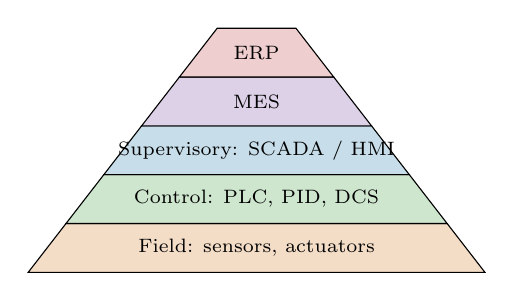
\begin{tikzpicture}[font=\scriptsize]
					\def\h{0.62}
					\foreach \i/\lab/\col in {
						0/{Field: sensors, actuators}/cOrange,
						1/{Control: PLC, PID, DCS}/cGreen,
						2/{Supervisory: SCADA / HMI}/cAccent,
						3/{MES}/cPurple,
						4/{ERP}/cRed} {
						\pgfmathsetmacro{\yb}{\i*\h}
						\pgfmathsetmacro{\yt}{(\i+1)*\h}
						\pgfmathsetmacro{\wb}{2.9-0.48*\i}
						\pgfmathsetmacro{\wt}{2.9-0.48*(\i+1)}
						\filldraw[draw=black, fill=\col!22] (-\wb,\yb) -- (\wb,\yb) -- (\wt,\yt) -- (-\wt,\yt) -- cycle;
						\node at (0,{(\i+0.5)*\h}) {\lab};
					}
				\end{tikzpicture}

				\footnotesize This course: the bottom three levels.
			\end{column}
		\end{columns}
	\end{frame}

	% =================================================================
	\section{Implementation of Digital Controllers}
	% =================================================================
	\begin{frame}{The Digital Control Loop}
		\centering
		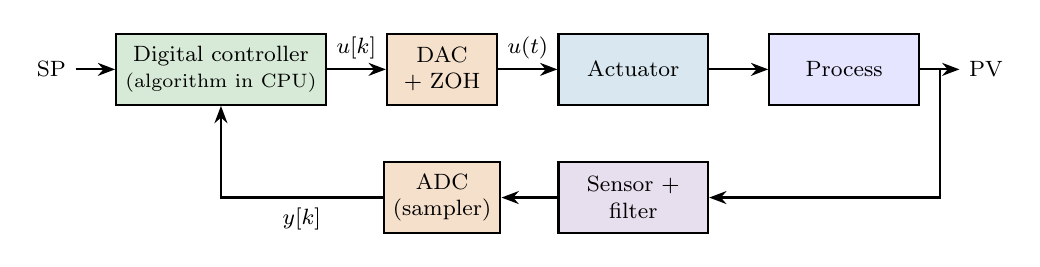
\begin{tikzpicture}[font=\footnotesize, node distance=0.75cm]
			\node (r) {SP};
			\node[blk, right=0.5cm of r, fill=cGreen!18, minimum width=2.3cm] (c) {Digital controller\\ \scriptsize(algorithm in CPU)};
			\node[blk, right=of c, fill=cOrange!20, minimum width=1.4cm] (dac) {DAC\\ + ZOH};
			\node[blk, right=of dac, fill=cAccent!15] (a) {Actuator};
			\node[blk, right=of a, fill=blue!10] (p) {Process};
			\node[right=0.5cm of p] (y) {PV};
			\node[blk, below=0.7cm of dac, fill=cOrange!20, minimum width=1.4cm] (adc) {ADC\\ (sampler)};
			\node[blk, below=0.7cm of a, fill=cPurple!15] (s) {Sensor +\\ filter};
			\draw[sig] (r) -- (c);
			\draw[sig] (c) -- node[above] {$u[k]$} (dac);
			\draw[sig] (dac) -- node[above] {$u(t)$} (a);
			\draw[sig] (a) -- (p);
			\draw[sig] (p) -- coordinate[pos=0.5] (tap) (y);
			\draw[sig] (tap) |- (s);
			\draw[sig] (s) -- (adc);
			\draw[sig] (adc) -| node[pos=0.25, below] {$y[k]$} (c);
		\end{tikzpicture}
		\vspace{0.25cm}
		\begin{itemize}\small
			\item The computer only sees the process at \textbf{sampling instants} $t = kT$ ($T$ = sample time).
			\item \textbf{ADC} converts the analog measurement to a number; \textbf{DAC} converts the output back.
			\item \textbf{Zero-order hold (ZOH)} keeps the output constant between samples $\rightarrow$ a ``staircase'' signal.
			\item Everything in between (filtering, PID, limits) is \textbf{software} --- easy to change and tune.
		\end{itemize}
	\end{frame}

	\begin{frame}{Sampling and Quantisation}
		\begin{columns}[T]
			\begin{column}{0.5\textwidth}
				\begin{block}{Quantisation (ADC resolution)}
					\small An $n$-bit ADC with full-scale range FSR has step
					\[
					q = \frac{\text{FSR}}{2^n}
					\]
					\textbf{Example:} 12-bit ADC, 0--10 V:\\
					$q = 10/4096 = \boxed{2.44\ \text{mV}}$
				\end{block}
				\begin{block}{Choosing the sample time $T$}
					\small Rule of thumb: $T \le \tau/10$ (process time constant) or 10--20 samples per rise time.
				\end{block}
			\end{column}
			\begin{column}{0.5\textwidth}
				\begin{block}{Aliasing \& Nyquist}
					\small Sample at least \textbf{twice} the highest signal frequency ($f_s > 2f_{\max}$), and use an analog \textbf{anti-aliasing filter} before the ADC --- otherwise fast noise appears as a false slow signal.
				\end{block}
				\centering
				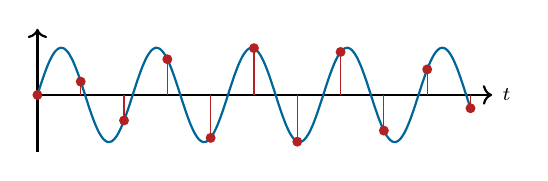
\begin{tikzpicture}[font=\scriptsize, x=0.55cm, y=0.6cm]
					\draw[->, thick] (0,0) -- (10.5,0) node[right] {$t$};
					\draw[->, thick] (0,-1.2) -- (0,1.4);
					\draw[cAccent, thick, domain=0:10, samples=100, smooth] plot (\x, {sin(deg(2*pi*\x/2.2))});
					\foreach \k in {0,...,10} {
						\pgfmathsetmacro{\v}{sin(deg(2*pi*\k/2.2))}
						\draw[cRed] (\k,0) -- (\k,\v);
						\fill[cRed] (\k,\v) circle (1.8pt);
					}
				\end{tikzpicture}

				\footnotesize Samples (red) of a continuous signal (blue).
			\end{column}
		\end{columns}
	\end{frame}

	\begin{frame}{Discrete PID: Position and Velocity Forms}
		\begin{columns}[T]
			\begin{column}{0.5\textwidth}
				\begin{block}{Position form}
					\small
					\[
					u[k] = K_p e[k] + K_i T\sum_{j=0}^{k} e[j] + \frac{K_d}{T}\big(e[k]-e[k-1]\big)
					\]
					Computes the \textbf{whole} output every sample; needs a separate anti-windup.
				\end{block}
			\end{column}
			\begin{column}{0.5\textwidth}
				\begin{block}{Velocity (incremental) form}
					\small
					\[
					\begin{aligned}
						\Delta u[k] &= K_p\big(e[k]-e[k-1]\big) + K_i T\,e[k]\\
						&\quad + \frac{K_d}{T}\big(e[k]-2e[k-1]+e[k-2]\big)\\
						u[k] &= u[k-1] + \Delta u[k]
					\end{aligned}
					\]
					Computes only the \textbf{change}.
				\end{block}
			\end{column}
		\end{columns}
		\vspace{0.2cm}
		\begin{block}{Why industry likes the velocity form}
			\small \textbf{No integral windup} (just clamp $u$ between 0 and 100\,\%), \textbf{bumpless} MANUAL$\leftrightarrow$AUTO transfer, and it suits stepper-motor valves that take \emph{increments}.
		\end{block}
	\end{frame}

	\begin{frame}{Digital Filtering of Measurements}
		\begin{columns}[T]
			\begin{column}{0.5\textwidth}
				\begin{block}{First-order low-pass filter}
					\small
					\[
					y_f[k] = a\,y_f[k-1] + (1-a)\,x[k],
					\qquad a = e^{-T/\tau_f}
					\]
					Smooths noisy measurements before the controller (especially before D action).
				\end{block}
				\textbf{Example:} $T = 0.1$ s, $\tau_f = 1$ s:
				\[
				a = e^{-0.1} = 0.905
				\]
				$y_f[k] = 0.905\,y_f[k-1] + 0.095\,x[k]$
			\end{column}
			\begin{column}{0.5\textwidth}
				\centering
				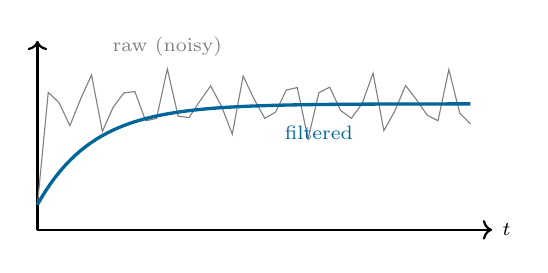
\begin{tikzpicture}[font=\scriptsize, x=0.55cm, y=1.6cm]
					\draw[->, thick] (0,0) -- (10.5,0) node[right] {$t$};
					\draw[->, thick] (0,0) -- (0,1.5);
					\draw[gray, thin] (0,0.2) \foreach \k in {1,...,40} { -- ({\k/4}, {1.0 + 0.18*sin(\k*97) + 0.1*cos(\k*151)})};
					\draw[very thick, cAccent, domain=0:10, samples=80, smooth] plot (\x, {1 - 0.8*exp(-\x/1.3)});
					\node[gray, above] at (3,1.3) {raw (noisy)};
					\node[cAccent, below] at (6.5,0.9) {filtered};
				\end{tikzpicture}
				\vspace{0.1cm}

				\footnotesize Larger $\tau_f$ = smoother, but \textbf{slower} (adds lag to the loop).
			\end{column}
		\end{columns}
	\end{frame}

	\begin{frame}{How a Digital Controller Runs: The Sample Cycle}
		\vspace*{-0.3cm}
		\begin{block}{The Tick---Read---Compute---Write cycle}
			Like the CPU's machine cycle, a digital controller repeats one fixed cycle,
			started by a \textbf{timer interrupt} every sample time $T$.
		\end{block}
		\begin{columns}[T]
			\begin{column}{0.55\textwidth}
				\begin{enumerate}\small
					\item \textbf{Tick} --- hardware timer interrupt every $T$ (fixed, not ``when ready'').
					\item \textbf{Read} --- start ADC, read PV; check for sensor fault.
					\item \textbf{Filter} --- digital low-pass filter on PV.
					\item \textbf{Compute} --- PID (velocity form), clamp 0--100\,\%.
					\item \textbf{Write} --- output to DAC; save $e[k]$, $e[k-1]$; wait for next tick.
				\end{enumerate}
			\end{column}
			\begin{column}{0.45\textwidth}
				\centering
				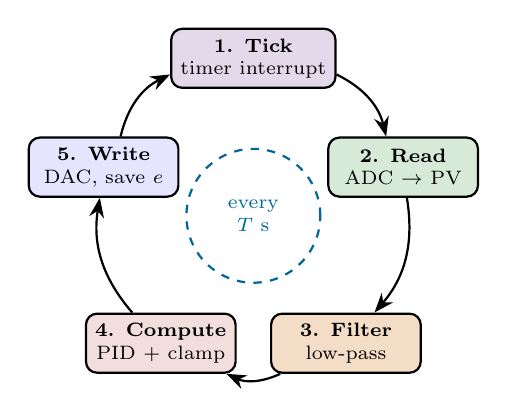
\begin{tikzpicture}[font=\scriptsize,
					stage/.style={rectangle, rounded corners=4pt, draw=black, thick,
						minimum width=1.9cm, minimum height=0.75cm, align=center}]
					\node[circle, draw=cAccent, thick, dashed, minimum size=1.7cm, align=center, text=cAccent]
					(c) at (0,0) {every\\ $T$ s};
					\node[stage, fill=cPurple!18] (t) at (90:2.0)   {\textbf{1. Tick}\\ timer interrupt};
					\node[stage, fill=cGreen!18]  (r) at (18:2.0)   {\textbf{2. Read}\\ ADC $\to$ PV};
					\node[stage, fill=cOrange!22] (f) at (-54:2.0)  {\textbf{3. Filter}\\ low-pass};
					\node[stage, fill=cRed!15]    (p) at (-126:2.0) {\textbf{4. Compute}\\ PID + clamp};
					\node[stage, fill=blue!10]    (w) at (162:2.0)  {\textbf{5. Write}\\ DAC, save $e$};
					\draw[flowarrow] (t) to[bend left=25] (r);
					\draw[flowarrow] (r) to[bend left=25] (f);
					\draw[flowarrow] (f) to[bend left=25] (p);
					\draw[flowarrow] (p) to[bend left=25] (w);
					\draw[flowarrow] (w) to[bend left=25] (t);
				\end{tikzpicture}
			\end{column}
		\end{columns}
	\end{frame}

	\begin{frame}[fragile, plain]{}

		\vspace*{0.05cm}

		\begin{columns}[T,onlytextwidth]

			% =========================================================
			% LEFT COLUMN -- PSEUDOCODE
			% =========================================================

			\begin{column}{0.25\textwidth}

				\begin{block}{Pseudocode}
					\scriptsize
					\begin{enumerate}
						\item START; $K_p = 2$, $K_i = 0.5$, $T = 1$ s
						\item SP $= 60\,^\circ$C, PV $= 20\,^\circ$C, $u = 0$
						\item \textbf{REPEAT} every $T$
						\begin{itemize}\scriptsize
							\item \texttt{e0 = SP - PV}
							\item \texttt{du} from velocity PID
							\item \texttt{u = u + du}
							\item clamp \texttt{u} to 0--100\,\%
							\item plant responds; shift \texttt{e2 = e1}, \texttt{e1 = e0}
						\end{itemize}
						\item STOP after 40 s
					\end{enumerate}
				\end{block}

			\end{column}


			% =========================================================
			% MIDDLE COLUMN -- C PROGRAM
			% =========================================================
			\hspace*{0.3cm}
			\begin{column}{0.48\textwidth}

				\begin{block}{C Program (velocity-form PID)}

\begin{lstlisting}[style=cstyle,numbers=none,basicstyle=\ttfamily\scriptsize]
#include <stdio.h>

int main(void)
{
	float Kp = 2.0, Ki = 0.5, Kd = 0.0, T = 1.0;
	float sp = 60.0, pv = 20.0, u = 0.0;
	float e0, e1 = 0.0, e2 = 0.0, du;
	int k;

	for (k = 1; k <= 40; k++) {
		e0 = sp - pv;
		du = Kp*(e0 - e1) + Ki*T*e0
		   + Kd/T*(e0 - 2*e1 + e2);
		u += du;
		if (u > 100.0) u = 100.0;   /* clamp */
		if (u < 0.0)   u = 0.0;
		pv += 0.1*(0.8*u + 20.0 - pv); /* plant */
		e2 = e1;  e1 = e0;
		if (k % 8 == 0)
			printf("t=%2d u=%5.1f PV=%5.1f\n",
			       k, u, pv);
	}
	return 0;
}
\end{lstlisting}

				\end{block}

			\end{column}


			% =========================================================
			% RIGHT COLUMN -- OUTPUT
			% =========================================================

			\begin{column}{0.25\textwidth}

				\begin{tikzpicture}[remember picture,overlay]
					\node[
					anchor=north east,
					draw,
					rounded corners=2pt,
					fill=white,
					text width=3.5cm,
					align=left,
					inner sep=6pt
					] at ([xshift=-2mm,yshift=-6mm]current page.north east)
					{
						\textbf{Program Output}\\[3pt]
						\ttfamily\scriptsize
						t= 8 u= 75.6 PV= 60.3\\
						t=16 u= 50.8 PV= 63.7\\
						t=24 u= 47.9 PV= 60.7\\
						t=32 u= 49.5 PV= 59.8\\
						t=40 u= 50.1 PV= 59.9\\[3pt]
						\sffamily (\texttt{t} in s, \texttt{u} in \%, PV in $^\circ$C)
					};
				\end{tikzpicture}

			\end{column}

		\end{columns}

		\begin{tikzpicture}[remember picture,overlay]
			\node[
			anchor=south east,
			draw,
			rounded corners=2pt,
			fill=cGrayBg,
			text width=3.5cm,
			align=left,
			inner sep=6pt,
			font=\scriptsize
			] at ([xshift=-2mm,yshift=4mm]current page.south east)
			{
				\textbf{Note:} the plant is a first-order heater model ($0.8\,^\circ$C per \% output, ambient $20\,^\circ$C). PV overshoots slightly, then settles at the 60\,$^\circ$C setpoint with about 50\,\% heater output. Because only \texttt{du} is added, clamping \texttt{u} is all the anti-windup needed.
			};
		\end{tikzpicture}

	\end{frame}

	% =================================================================
	\section{Control Strategies for Industrial Processes}
	% =================================================================
	\begin{frame}{Overview of Control Strategies}
		\renewcommand{\arraystretch}{1.25}
		\centering
		\small
		\begin{tabular}{@{}>{\raggedright}p{2.8cm}>{\raggedright}p{5.4cm}>{\raggedright\arraybackslash}p{4.4cm}@{}}
			\toprule
			\textbf{Strategy} & \textbf{Idea} & \textbf{Typical use} \\
			\midrule
			ON--OFF          & output 0 or 100\,\% with a dead band & tank heaters, bilge pumps \\
			Feedback (PID)   & correct the measured error            & most single loops \\
			Feedforward      & act on a \emph{measured disturbance} before it upsets PV & boiler feedwater, heat exchangers \\
			Cascade          & outer loop sets the SP of a fast inner loop & jacket temperature, valve flow \\
			Ratio            & keep one flow a fixed ratio of another & fuel/air, blending \\
			Split-range      & one controller drives two valves        & heating \& cooling \\
			Override / selector & the more critical of two controllers wins & compressor surge, limits \\
			Advanced (MPC, adaptive) & model-based, multivariable, self-tuning & refineries, ship autopilots \\
			\bottomrule
		\end{tabular}
	\end{frame}

	\begin{frame}{Feedforward Control}
		\begin{columns}[T]
			\begin{column}{0.5\textwidth}
				\begin{block}{Idea}
					\small Feedback waits until the disturbance has \textbf{already} changed PV. Feedforward \textbf{measures the disturbance} and corrects the output immediately. Feedback trims what feedforward misses.
				\end{block}
				\begin{itemize}\small
					\item Needs a measurable disturbance and a model of its effect.
					\item Almost always used \textbf{with} feedback, never alone.
					\item Example: heat exchanger --- measure inlet flow change, adjust steam at once.
				\end{itemize}
			\end{column}
			\begin{column}{0.5\textwidth}
				\centering
				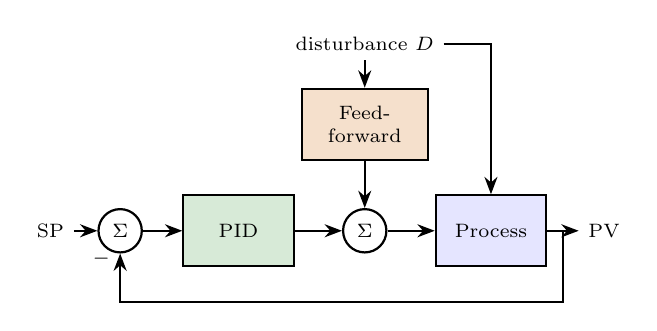
\begin{tikzpicture}[font=\scriptsize, node distance=0.55cm]
					\node[blk, fill=cOrange!20, minimum width=1.6cm] (ff) {Feed-\\ forward};
					\node[above=0.35cm of ff] (d) {disturbance $D$};
					\node[sumj, below=0.6cm of ff] (s2) {$\Sigma$};
					\node[blk, left=0.6cm of s2, fill=cGreen!18, minimum width=1.4cm] (fb) {PID};
					\node[sumj, left=0.5cm of fb] (s1) {$\Sigma$};
					\node[left=0.3cm of s1] (sp) {SP};
					\node[blk, right=0.6cm of s2, fill=blue!10, minimum width=1.4cm] (p) {Process};
					\node[right=0.4cm of p] (y) {PV};
					\draw[sig] (d) -- (ff);
					\draw[sig] (d) -| (p.north);
					\draw[sig] (ff) -- (s2);
					\draw[sig] (sp) -- (s1);
					\draw[sig] (s1) -- (fb);
					\draw[sig] (fb) -- (s2);
					\draw[sig] (s2) -- (p);
					\draw[sig] (p) -- coordinate[pos=0.5] (tap) (y);
					\draw[sig] (tap) -- ++(0,-0.9) -| node[pos=0.95, left] {$-$} (s1.south);
				\end{tikzpicture}
			\end{column}
		\end{columns}
	\end{frame}

	\begin{frame}{Cascade Control}
		\begin{columns}[T]
			\begin{column}{0.5\textwidth}
				\begin{block}{Idea}
					\small Two controllers in series: the \textbf{outer (master)} controller sets the setpoint of the \textbf{inner (slave)} controller. The fast inner loop kills disturbances before they reach the slow outer variable.
				\end{block}
				\begin{itemize}\small
					\item Inner loop must be \textbf{3--10$\times$ faster} than the outer.
					\item Tune the inner loop first, then the outer.
					\item Example: reactor temperature (outer) $\rightarrow$ cooling-water flow (inner).
				\end{itemize}
			\end{column}
			\begin{column}{0.5\textwidth}
				\centering
				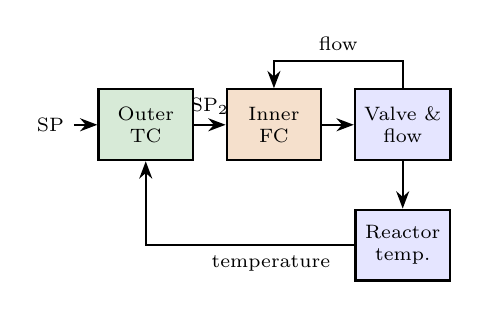
\begin{tikzpicture}[font=\scriptsize, node distance=0.4cm]
					\node (sp) {SP};
					\node[blk, right=0.3cm of sp, fill=cGreen!18, minimum width=1.2cm] (c1) {Outer\\ TC};
					\node[blk, right=of c1, fill=cOrange!20, minimum width=1.2cm] (c2) {Inner\\ FC};
					\node[blk, right=of c2, fill=blue!10, minimum width=1.2cm] (v) {Valve \&\\ flow};
					\node[blk, below=0.6cm of v, fill=blue!10, minimum width=1.2cm] (p) {Reactor\\ temp.};
					\draw[sig] (sp) -- (c1);
					\draw[sig] (c1) -- node[above] {SP$_2$} (c2);
					\draw[sig] (c2) -- (v);
					\draw[sig] (v) -- (p);
					\draw[sig] (v.north) -- ++(0,0.35) -| node[pos=0.25, above] {flow} (c2.north);
					\draw[sig] (p.west) -| node[pos=0.2, below] {temperature} (c1.south);
				\end{tikzpicture}
			\end{column}
		\end{columns}
	\end{frame}

	\begin{frame}{Ratio, Split-Range and Override Control}
		\begin{columns}[T]
			\begin{column}{0.5\textwidth}
				\begin{block}{Ratio control}
					\small Keep flow B at a fixed ratio $R$ of flow A: $\text{SP}_B = R \times F_A$.\\
					\textbf{Example:} boiler fuel flow 2 t/h, air/fuel ratio 15:1 $\Rightarrow$ air SP $= 15\times2 = \boxed{30\ \text{t/h}}$.
				\end{block}
				\begin{block}{Override (selector) control}
					\small Two controllers share one valve; a \textbf{low / high selector} passes the safer output --- e.g.\ a pressure limit overrides the flow controller.
				\end{block}
			\end{column}
			\begin{column}{0.5\textwidth}
				\begin{block}{Split-range control}
					\small One controller output drives \textbf{two} valves over different ranges of its signal.
				\end{block}
				\centering
				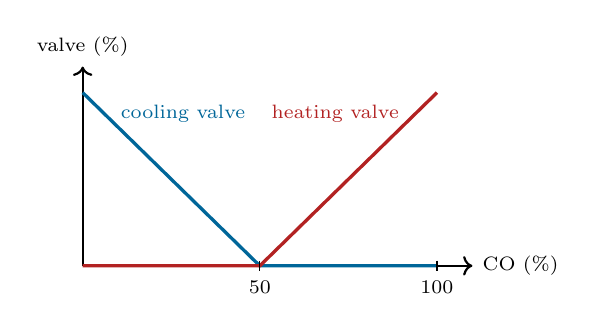
\begin{tikzpicture}[font=\scriptsize, x=0.045cm, y=0.022cm]
					\draw[->, thick] (0,0) -- (110,0) node[right] {CO (\%)};
					\draw[->, thick] (0,0) -- (0,115) node[above] {valve (\%)};
					\draw[very thick, cAccent] (0,100) -- (50,0) -- (100,0);
					\draw[very thick, cRed] (0,0) -- (50,0) -- (100,100);
					\foreach \x in {50,100} \draw (\x,3) -- (\x,-3) node[below] {\x};
					\node[cAccent, right] at (8,88) {cooling valve};
					\node[cRed, left] at (92,88) {heating valve};
				\end{tikzpicture}

				\footnotesize 0--50\,\%: cooling; 50--100\,\%: heating.
			\end{column}
		\end{columns}
	\end{frame}

	% =================================================================
	\section{Programmable Logic Controllers}
	% =================================================================
	\begin{frame}{PLC Architecture}
		\centering
		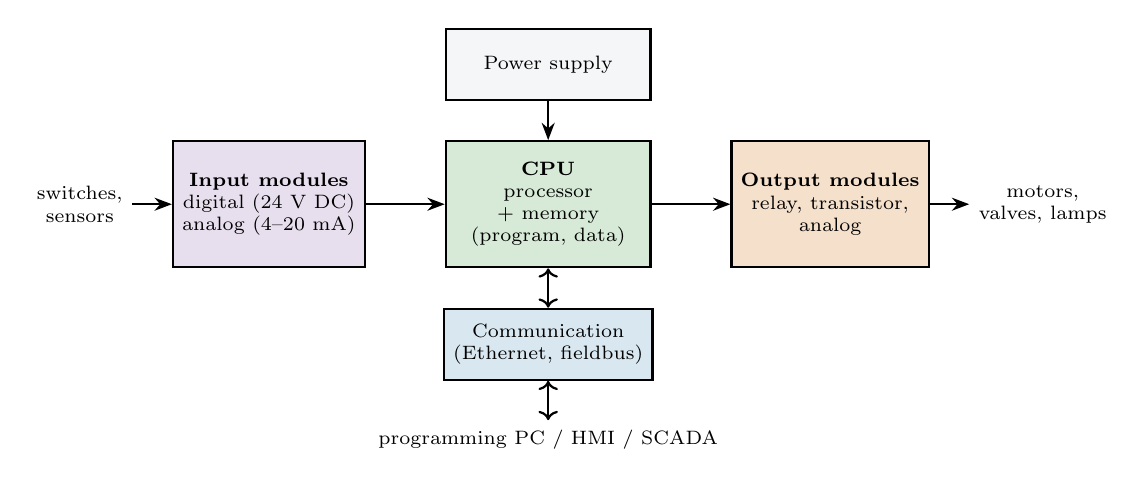
\begin{tikzpicture}[font=\scriptsize, node distance=0.5cm]
			\node[blk, fill=cGreen!18, minimum width=2.6cm, minimum height=1.6cm] (cpu) {\textbf{CPU}\\ processor\\ + memory\\ (program, data)};
			\node[blk, left=1.0cm of cpu, fill=cPurple!15, minimum width=2.2cm, minimum height=1.6cm] (in) {\textbf{Input modules}\\ digital (24 V DC)\\ analog (4--20 mA)};
			\node[blk, right=1.0cm of cpu, fill=cOrange!20, minimum width=2.2cm, minimum height=1.6cm] (out) {\textbf{Output modules}\\ relay, transistor,\\ analog};
			\node[blk, above=0.5cm of cpu, fill=cGrayBg, minimum width=2.6cm] (ps) {Power supply};
			\node[blk, below=0.5cm of cpu, fill=cAccent!15, minimum width=2.6cm] (com) {Communication\\ (Ethernet, fieldbus)};
			\node[left=0.5cm of in, align=center] (sw) {switches,\\ sensors};
			\node[right=0.5cm of out, align=center] (ld) {motors,\\ valves, lamps};
			\node[below=0.5cm of com] (pc) {programming PC / HMI / SCADA};
			\draw[sig] (sw) -- (in); \draw[sig] (in) -- (cpu); \draw[sig] (cpu) -- (out); \draw[sig] (out) -- (ld);
			\draw[sig] (ps) -- (cpu); \draw[<->, thick] (cpu) -- (com); \draw[<->, thick] (com) -- (pc);
		\end{tikzpicture}
		\vspace{0.15cm}
		\begin{itemize}\small
			\item \textbf{Rugged}: designed for heat, vibration, electrical noise --- unlike an office PC.
			\item \textbf{Modular}: add I/O cards as the machine grows; remote I/O over a network.
			\item \textbf{Safety PLCs} (redundant CPUs, self-tests) for emergency shutdown systems.
		\end{itemize}
	\end{frame}

	\begin{frame}{The PLC Scan Cycle and Response Time}
		\begin{columns}[T]
			\begin{column}{0.5\textwidth}
				\centering
				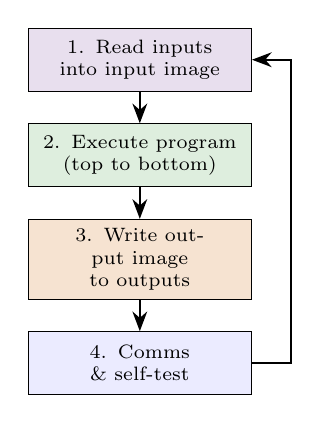
\begin{tikzpicture}[font=\scriptsize, node distance=0.4cm]
					\node[process, fill=cPurple!15, text width=2.6cm] (r) {1. Read inputs\\ into input image};
					\node[process, fill=cGreen!15, below=of r, text width=2.6cm] (e) {2. Execute program\\ (top to bottom)};
					\node[process, fill=cOrange!18, below=of e, text width=2.6cm] (w) {3. Write output image\\ to outputs};
					\node[process, fill=blue!8, below=of w, text width=2.6cm] (h) {4. Comms \& self-test};
					\draw[flowarrow] (r) -- (e); \draw[flowarrow] (e) -- (w); \draw[flowarrow] (w) -- (h);
					\draw[flowarrow] (h.east) -- ++(0.5,0) |- (r.east);
				\end{tikzpicture}
			\end{column}
			\begin{column}{0.5\textwidth}
				\begin{block}{Scan time}
					\small Typically 1--50 ms, depending on program size and CPU speed.
				\end{block}
				\begin{block}{Worst-case response time}
					\small An input can change just \emph{after} it was read, so it is seen one scan later and acted on at the end of the next:
					\[
					t_{\text{resp}} \approx t_{\text{in filter}} + 2\,t_{\text{scan}} + t_{\text{out}}
					\]
					\textbf{Example:} filter 3 ms, scan 5 ms, relay output 10 ms:\\
					$t_{\text{resp}} \approx 3 + 10 + 10 = \boxed{23\ \text{ms}}$
				\end{block}
			\end{column}
		\end{columns}
	\end{frame}

	\begin{frame}{PLC Programming Languages (IEC 61131-3)}
		\renewcommand{\arraystretch}{1.3}
		\centering
		\small
		\begin{tabular}{@{}>{\raggedright}p{3.4cm}cp{4.2cm}p{3.6cm}@{}}
			\toprule
			\textbf{Language} & \textbf{Type} & \textbf{Looks like} & \textbf{Best for} \\
			\midrule
			Ladder Diagram (LD)        & graphical & relay circuits, rungs  & simple logic, electricians \\
			Function Block Diagram (FBD) & graphical & connected blocks     & process \& analog control \\
			Structured Text (ST)       & text      & Pascal / C             & calculations, algorithms \\
			Sequential Function Chart (SFC) & graphical & steps \& transitions & sequences, batches \\
			Instruction List (IL)      & text      & assembly               & legacy (deprecated) \\
			\bottomrule
		\end{tabular}
		\vspace{0.3cm}
		\begin{block}{Key idea}
			\small All languages can be mixed in one project. The same logic can be written in LD or ST --- choose the one that is clearest for the people who will maintain it.
		\end{block}
	\end{frame}

	\begin{frame}[fragile]{Timers in Ladder Logic and Structured Text}
		\begin{columns}[T]
			\begin{column}{0.55\textwidth}
				\textbf{Conveyor starts 5 s after START (warning horn first)}
				\vspace{0.1cm}

				\centering
				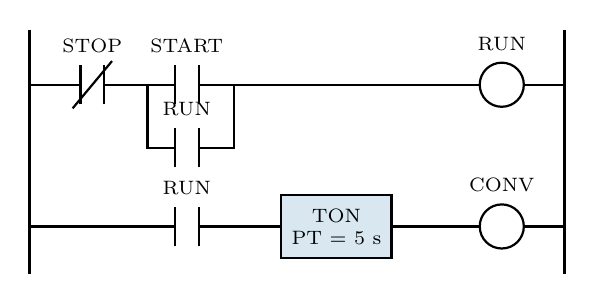
\begin{tikzpicture}[font=\scriptsize]
					\draw[very thick] (0,0.7) -- (0,-2.4);
					\draw[very thick] (6.8,0.7) -- (6.8,-2.4);
					% rung 1: latch RUN
					\draw[thick] (0,0) -- (0.65,0);
					\ladNC{0.8}{0}{STOP}
					\draw[thick] (0.95,0) -- (1.85,0);
					\ladNO{2.0}{0}{START}
					\draw[thick] (2.15,0) -- (5.72,0);
					\ladCoil{6.0}{0}{RUN}
					\draw[thick] (6.28,0) -- (6.8,0);
					\draw[thick] (1.5,0) -- (1.5,-0.8) -- (1.85,-0.8);
					\ladNO{2.0}{-0.8}{RUN}
					\draw[thick] (2.15,-0.8) -- (2.6,-0.8) -- (2.6,0);
					% rung 2: timer
					\draw[thick] (0,-1.8) -- (1.85,-1.8);
					\ladNO{2.0}{-1.8}{RUN}
					\draw[thick] (2.15,-1.8) -- (3.2,-1.8);
					\draw[thick, fill=cAccent!15] (3.2,-2.2) rectangle (4.6,-1.4);
					\node[align=center] at (3.9,-1.8) {TON\\ PT = 5 s};
					\draw[thick] (4.6,-1.8) -- (5.72,-1.8);
					\ladCoil{6.0}{-1.8}{CONV}
					\draw[thick] (6.28,-1.8) -- (6.8,-1.8);
				\end{tikzpicture}
			\end{column}
			\begin{column}{0.45\textwidth}
				\textbf{Same logic in Structured Text}
\begin{lstlisting}[style=ststyle]
(* latch the RUN flag *)
RUN := (START OR RUN) AND NOT STOP;

(* on-delay timer, 5 s *)
T1(IN := RUN, PT := T#5s);
CONV := T1.Q;
HORN := RUN AND NOT T1.Q;
\end{lstlisting}
				\footnotesize \textbf{TON} (on-delay): output \texttt{Q} turns ON when \texttt{IN} has been ON for the preset time \texttt{PT}. Counters (\textbf{CTU}, \textbf{CTD}) work the same way with pulses.
			\end{column}
		\end{columns}
	\end{frame}

	% =================================================================
	\section{Real-Time Issues in Signal Transmission and Control}
	% =================================================================
	\begin{frame}{What Does ``Real-Time'' Mean?}
		\begin{block}{Real-time system}
			A system whose correctness depends not only on the \textbf{result} but also on the \textbf{time} at which the result is produced. A late answer is a \emph{wrong} answer.
		\end{block}
		\begin{columns}[T]
			\begin{column}{0.32\textwidth}
				\begin{block}{Hard real-time}
					\small Missing a deadline = failure.\\ Airbag, ESD trip, motion control.
				\end{block}
			\end{column}
			\begin{column}{0.32\textwidth}
				\begin{block}{Firm real-time}
					\small Late results are useless but tolerated occasionally.\\ Video frames, some sampling.
				\end{block}
			\end{column}
			\begin{column}{0.32\textwidth}
				\begin{block}{Soft real-time}
					\small Late results lose value gradually.\\ HMI screens, trends, reports.
				\end{block}
			\end{column}
		\end{columns}
		\vspace{0.2cm}
		\begin{itemize}\small
			\item \textbf{Latency} --- delay from event to reaction. \quad \textbf{Jitter} --- variation of that delay.
			\item \textbf{Determinism} --- the worst-case time is known and guaranteed.
		\end{itemize}
	\end{frame}

	\begin{frame}{Latency, Jitter and their Effect on Control}
		\begin{columns}[T]
			\begin{column}{0.5\textwidth}
				\centering
				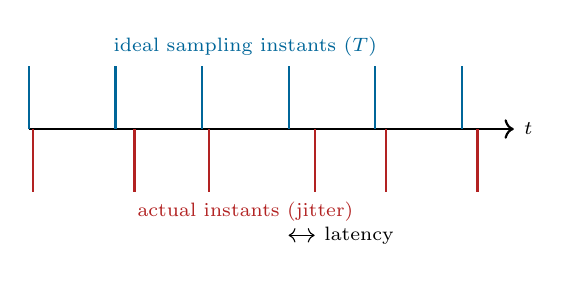
\begin{tikzpicture}[font=\scriptsize, x=1.1cm]
					\draw[->, thick] (0,0) -- (5.6,0) node[right] {$t$};
					\foreach \k in {0,...,5} {
						\draw[cAccent, thick] (\k,0) -- (\k,0.8);
					}
					\node[cAccent, above] at (2.5,0.8) {ideal sampling instants ($T$)};
					\foreach \k/\d in {0/0.05,1/0.22,2/0.08,3/0.3,4/0.12,5/0.18} {
						\draw[cRed, thick] ({\k+\d},0) -- ({\k+\d},-0.8);
					}
					\node[cRed, below] at (2.5,-0.8) {actual instants (jitter)};
					\draw[<->] (3,-1.35) -- (3.3,-1.35) node[right] {latency};
				\end{tikzpicture}
			\end{column}
			\begin{column}{0.5\textwidth}
				\begin{block}{Delay costs phase margin}
					\small A pure time delay $\tau_d$ adds a phase lag of $\omega\tau_d$ (rad) at frequency $\omega$ --- the loop moves closer to instability.
				\end{block}
				\textbf{Example:} crossover frequency $\omega_c = 10$ rad/s, network + computing delay $\tau_d = 20$ ms:
				\[
				\phi = 10\times0.02 = 0.2\ \text{rad} \approx \boxed{11.5^\circ}
				\]
				\footnotesize If the loop had 45$^\circ$ phase margin, only $\approx$33.5$^\circ$ remain --- more overshoot.
			\end{column}
		\end{columns}
	\end{frame}

	\begin{frame}{Scheduling Real-Time Tasks}
		\begin{columns}[T]
			\begin{column}{0.5\textwidth}
				\begin{block}{Rate-monotonic scheduling}
					\small Periodic tasks; the task with the \textbf{shortest period} gets the \textbf{highest priority}. A set of $n$ tasks is guaranteed to meet all deadlines if
					\[
					U = \sum_{i=1}^{n}\frac{C_i}{T_i} \;\le\; n\left(2^{1/n} - 1\right)
					\]
					$C_i$ = execution time, $T_i$ = period.
				\end{block}
			\end{column}
			\begin{column}{0.5\textwidth}
				\renewcommand{\arraystretch}{1.2}
				\centering
				\small
				\begin{tabular}{@{}lccc@{}}
					\toprule
					\textbf{Task} & $\bm{C}$ (ms) & $\bm{T}$ (ms) & $\bm{C/T}$ \\
					\midrule
					Fast PID loop    & 1 & 10 & 0.10 \\
					Slow PID loops   & 2 & 20 & 0.10 \\
					Logic \& comms   & 6 & 40 & 0.15 \\
					\midrule
					\textbf{Total} $U$ & & & \textbf{0.35} \\
					\bottomrule
				\end{tabular}
				\vspace{0.2cm}

				\small Bound for $n = 3$: $3(2^{1/3}-1) = 0.78$\\
				$0.35 \le 0.78$ $\Rightarrow$ \textbf{schedulable} \checkmark
			\end{column}
		\end{columns}
		\vspace{0.1cm}
		\footnotesize\centering A \textbf{watchdog timer} resets the controller (or trips to a safe state) if the program ever stops completing its cycle on time.
	\end{frame}

	\begin{frame}{Signal Transmission Issues}
		\begin{columns}[T]
			\begin{column}{0.5\textwidth}
				\begin{block}{Noise and interference}
					\begin{itemize}\small
						\item \textbf{EMI} from motors, VFDs, radios, welding.
						\item \textbf{Ground loops} --- two earth points at different potentials.
						\item Cable \textbf{resistance} and voltage drop on long runs.
					\end{itemize}
				\end{block}
				\begin{block}{Good practice}
					\begin{itemize}\small
						\item Shielded twisted-pair cable; shield earthed at \emph{one} end.
						\item Separate signal and power cable trays.
						\item Galvanic isolation (isolators, optocouplers).
					\end{itemize}
				\end{block}
			\end{column}
			\begin{column}{0.5\textwidth}
				\renewcommand{\arraystretch}{1.25}
				\centering
				\small
				\begin{tabular}{@{}>{\raggedright}p{2.2cm}>{\raggedright\arraybackslash}p{3.6cm}@{}}
					\toprule
					\textbf{Signal} & \textbf{Property} \\
					\midrule
					0--10 V      & simple, but voltage drop \& noise on long cables \\
					4--20 mA     & current is the same all round the loop; live zero detects broken wire \\
					HART         & digital data on top of 4--20 mA \\
					Fieldbus / Ethernet & many values on one cable, diagnostics \\
					Fibre optic  & immune to EMI, long distances \\
					\bottomrule
				\end{tabular}
			\end{column}
		\end{columns}
	\end{frame}

	% =================================================================
	\section{Communication Systems for Industrial Automation}
	% =================================================================
	\begin{frame}{Industrial Network Hierarchy}
		\centering
		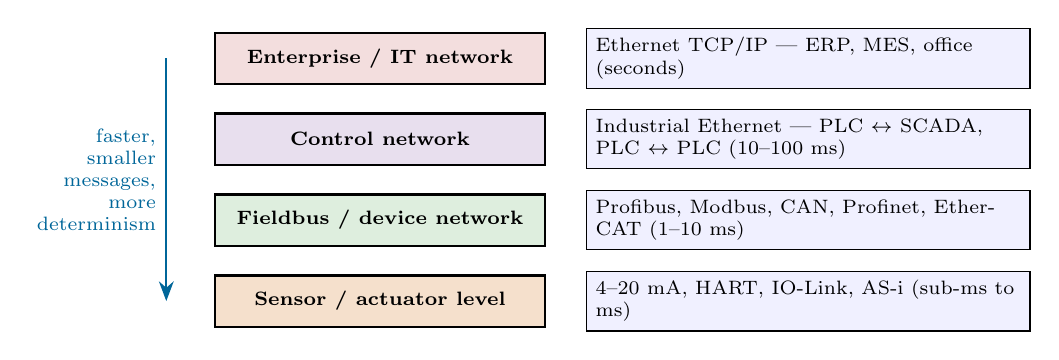
\begin{tikzpicture}[font=\scriptsize, node distance=0.35cm,
			lvl/.style={rectangle, draw=black, thick, minimum width=4.2cm, minimum height=0.65cm, align=center},
			ex/.style={rectangle, draw=black, fill=blue!6, text width=5.4cm, minimum height=0.65cm, align=left}]
			\node[lvl, fill=cRed!15] (l4) {\textbf{Enterprise / IT network}};
			\node[lvl, fill=cPurple!15, below=of l4] (l3) {\textbf{Control network}};
			\node[lvl, fill=cGreen!15, below=of l3] (l2) {\textbf{Fieldbus / device network}};
			\node[lvl, fill=cOrange!20, below=of l2] (l1) {\textbf{Sensor / actuator level}};
			\node[ex, right=0.5cm of l4] {Ethernet TCP/IP --- ERP, MES, office (seconds)};
			\node[ex, right=0.5cm of l3] {Industrial Ethernet --- PLC $\leftrightarrow$ SCADA, PLC $\leftrightarrow$ PLC (10--100 ms)};
			\node[ex, right=0.5cm of l2] {Profibus, Modbus, CAN, Profinet, EtherCAT (1--10 ms)};
			\node[ex, right=0.5cm of l1] {4--20 mA, HART, IO-Link, AS-i (sub-ms to ms)};
			\draw[flowarrow, cAccent] ($(l4.west)+(-0.6,0)$) -- ($(l1.west)+(-0.6,0)$) node[midway, left, align=right] {faster,\\ smaller\\ messages,\\ more\\ determinism};
		\end{tikzpicture}
		\vspace{0.2cm}

		\small Upper levels move \textbf{large amounts of data}; lower levels move \textbf{small data very fast and predictably}.
	\end{frame}

	\begin{frame}{Topologies and Medium Access}
		\begin{columns}[T]
			\begin{column}{0.55\textwidth}
				\centering
				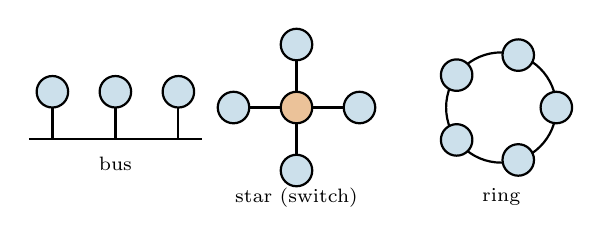
\begin{tikzpicture}[font=\scriptsize, nd/.style={circle, draw, thick, fill=cAccent!20, minimum size=0.4cm, inner sep=0pt}]
					% bus
					\begin{scope}[shift={(0,0)}]
						\draw[thick] (0,0) -- (2.2,0);
						\foreach \x in {0.3,1.1,1.9} {\draw[thick] (\x,0) -- (\x,0.4); \node[nd] at (\x,0.6) {};}
						\node[below] at (1.1,-0.1) {bus};
					\end{scope}
					% star
					\begin{scope}[shift={(3.4,0.4)}]
						\node[nd, fill=cOrange!40] (h) at (0,0) {};
						\foreach \a in {0,90,180,270} {\node[nd] (n\a) at (\a:0.8) {}; \draw[thick] (h) -- (n\a);}
						\node[below] at (0,-0.9) {star (switch)};
					\end{scope}
					% ring
					\begin{scope}[shift={(6.0,0.4)}]
						\draw[thick] (0,0) circle (0.7);
						\foreach \a in {0,72,...,288} \node[nd] at (\a:0.7) {};
						\node[below] at (0,-0.9) {ring};
					\end{scope}
				\end{tikzpicture}
				\vspace{0.2cm}

				\small Ring topologies with \textbf{media redundancy} keep running if one cable is cut --- common on ships.
			\end{column}
			\begin{column}{0.45\textwidth}
				\begin{block}{Who talks when? (medium access)}
					\small
					\textbf{Master--slave (polling)} --- master asks each slave in turn; deterministic (Modbus, Profibus DP).\\[3pt]
					\textbf{Token passing} --- a token circulates; only its holder transmits.\\[3pt]
					\textbf{CSMA} --- listen, then talk; collisions resolved by priority (CAN) or switches (Ethernet).\\[3pt]
					\textbf{Time-slot (TDMA)} --- each node owns a fixed time window (EtherCAT, TSN).
				\end{block}
			\end{column}
		\end{columns}
	\end{frame}

	\begin{frame}{Common Industrial Protocols}
		\renewcommand{\arraystretch}{1.2}
		\centering
		\small
		\begin{tabular}{@{}>{\raggedright}p{2.6cm}>{\raggedright}p{2.8cm}>{\raggedright}p{3.4cm}>{\raggedright\arraybackslash}p{3.8cm}@{}}
			\toprule
			\textbf{Protocol} & \textbf{Medium} & \textbf{Access} & \textbf{Typical use} \\
			\midrule
			Modbus RTU / TCP   & RS-485 / Ethernet & master--slave, polling  & simple, universal; meters, drives \\
			Profibus DP        & RS-485            & token + master--slave   & factory \& process I/O \\
			CAN / CANopen      & twisted pair      & CSMA with priority      & machines, vehicles \\
			NMEA 2000          & CAN               & CSMA with priority      & ship navigation \& engine data \\
			HART               & on 4--20 mA       & master--slave           & smart field instruments \\
			Profinet, EtherNet/IP & Ethernet       & switched, real-time classes & modern PLC systems \\
			EtherCAT           & Ethernet          & on-the-fly frame processing & fast motion control \\
			\bottomrule
		\end{tabular}
		\vspace{0.2cm}

		\footnotesize\centering Wireless options (WirelessHART, ISA100, Wi-Fi, 5G) are used for monitoring more than for fast control.
	\end{frame}

	\begin{frame}{Modbus RTU: Frame and Timing Worked Example}
		\begin{block}{Request frame: ``slave 1, read 2 holding registers from address 0''}
			\centering
			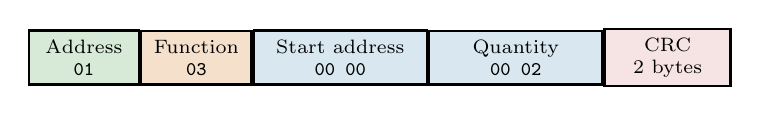
\begin{tikzpicture}[font=\scriptsize, fb/.style={rectangle, draw, thick, minimum height=0.6cm, align=center}]
				\node[fb, fill=cGreen!18, minimum width=1.4cm] (a) {Address\\ \texttt{01}};
				\node[fb, fill=cOrange!20, minimum width=1.4cm, right=0cm of a] (b) {Function\\ \texttt{03}};
				\node[fb, fill=cAccent!15, minimum width=2.2cm, right=0cm of b] (c) {Start address\\ \texttt{00 00}};
				\node[fb, fill=cAccent!15, minimum width=2.2cm, right=0cm of c] (d) {Quantity\\ \texttt{00 02}};
				\node[fb, fill=cRed!12, minimum width=1.6cm, right=0cm of d] (e) {CRC\\ 2 bytes};
			\end{tikzpicture}
		\end{block}
		\begin{columns}[T]
			\begin{column}{0.5\textwidth}
				\textbf{Problem:} RS-485 at 19\,200 baud, 11 bits per byte (start + 8 data + parity + stop). Request = 8 bytes, reply = 9 bytes, silent gap of 3.5 characters before each frame. How long is one poll?
			\end{column}
			\begin{column}{0.5\textwidth}
				\small
				\begin{align*}
					t_{\text{req}} &= \tfrac{8\times11}{19\,200} = 4.58\ \text{ms}\\
					t_{\text{rep}} &= \tfrac{9\times11}{19\,200} = 5.16\ \text{ms}\\
					t_{\text{gap}} &= \tfrac{3.5\times11}{19\,200} = 2.01\ \text{ms}\ (\times2)\\
					t_{\text{poll}} &\approx \boxed{13.8\ \text{ms}} \;\Rightarrow\; \approx 72\ \text{polls/s}
				\end{align*}
			\end{column}
		\end{columns}
		\vspace{0.1cm}
		\footnotesize\centering With 10 slaves each device is refreshed only $\sim$7 times per second --- fine for monitoring, too slow for fast control loops.
	\end{frame}

	% =================================================================
	\section{Data Acquisition and Supervisory Control}
	% =================================================================
	\begin{frame}{Data Acquisition (DAQ) Systems}
		\centering
		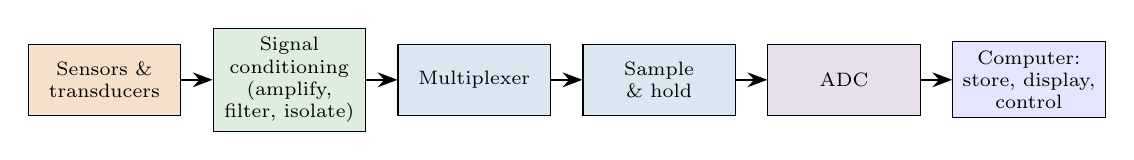
\begin{tikzpicture}[every node/.style={font=\scriptsize}, node distance=0.4cm,
			st/.style={process, minimum width=1.7cm, text width=1.7cm, minimum height=0.9cm}]
			\node[st, fill=cOrange!20] (s) {Sensors \& transducers};
			\node[st, right=of s, fill=cGreen!15] (c) {Signal conditioning (amplify, filter, isolate)};
			\node[st, right=of c, fill=cAccent!15] (m) {Multiplexer};
			\node[st, right=of m, fill=cAccent!15] (sh) {Sample \& hold};
			\node[st, right=of sh, fill=cPurple!15] (a) {ADC};
			\node[st, right=of a, fill=blue!10] (pc) {Computer: store, display, control};
			\draw[flowarrow] (s) -- (c); \draw[flowarrow] (c) -- (m); \draw[flowarrow] (m) -- (sh); \draw[flowarrow] (sh) -- (a); \draw[flowarrow] (a) -- (pc);
		\end{tikzpicture}
		\vspace{0.3cm}
		\begin{columns}[T]
			\begin{column}{0.5\textwidth}
				\begin{itemize}\small
					\item One ADC is shared by many channels through the \textbf{multiplexer}.
					\item \textbf{Sample \& hold} freezes the signal during conversion.
					\item Specs: channels, resolution (bits), sample rate, accuracy, isolation.
				\end{itemize}
			\end{column}
			\begin{column}{0.5\textwidth}
				\begin{block}{Worked example}
					\small 16 temperature channels, each sampled at 100 Hz, 16-bit ADC:\\
					aggregate rate $= 16\times100 = \boxed{1600\ \text{S/s}}$\\
					data rate $= 1600\times2\ \text{bytes} = 3.2$ kB/s $\approx 276$ MB/day.
				\end{block}
			\end{column}
		\end{columns}
	\end{frame}

	\begin{frame}{SCADA Architecture}
		\centering
		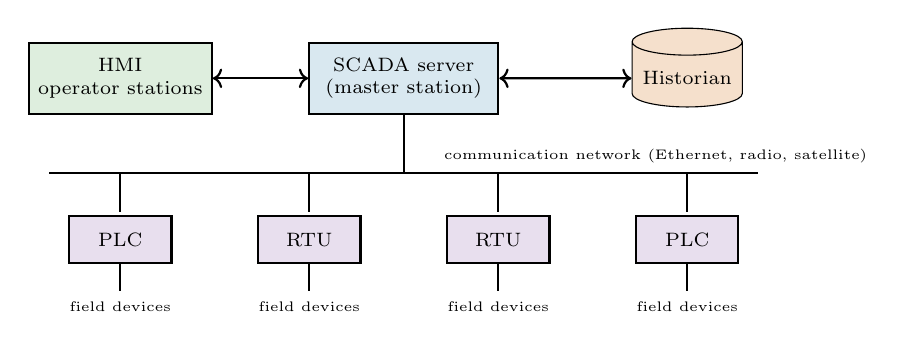
\begin{tikzpicture}[font=\scriptsize]
			\node[blk, fill=cAccent!15, minimum width=2.4cm] (ms) at (0,2.6) {SCADA server\\ (master station)};
			\node[blk, fill=cGreen!15, minimum width=1.8cm] (hmi) at (-3.6,2.6) {HMI\\ operator stations};
			\node[cylinder, draw=black, shape border rotate=90, aspect=0.25, minimum width=1.4cm, minimum height=1.0cm, fill=cOrange!20, align=center] (hist) at (3.6,2.6) {Historian};
			\draw[<->, thick] (hmi) -- (ms); \draw[<->, thick] (ms) -- (hist);
			\draw[thick] (-4.5,1.4) -- (4.5,1.4);
			\node[above, font=\tiny] at (3.2,1.4) {communication network (Ethernet, radio, satellite)};
			\draw[thick] (ms) -- (0,1.4);
			\foreach \x/\n in {-3.6/PLC, -1.2/RTU, 1.2/RTU, 3.6/PLC} {
				\draw[thick] (\x,1.4) -- (\x,0.9);
				\node[blk, fill=cPurple!15, minimum width=1.3cm, minimum height=0.6cm] at (\x,0.55) {\n};
				\draw[thick] (\x,0.25) -- (\x,-0.1);
				\node[font=\tiny] at (\x,-0.3) {field devices};
			}
		\end{tikzpicture}
		\vspace{0.2cm}
		\begin{columns}[T]
			\begin{column}{0.5\textwidth}
				\begin{itemize}\small
					\item \textbf{RTU / PLC} --- collect field data, run local control.
					\item \textbf{Master station} --- polls RTUs, stores data, runs logic.
				\end{itemize}
			\end{column}
			\begin{column}{0.5\textwidth}
				\begin{itemize}\small
					\item \textbf{HMI} --- mimic diagrams, alarms, trends, commands.
					\item \textbf{Historian} --- long-term data for reports \& analysis.
				\end{itemize}
			\end{column}
		\end{columns}
	\end{frame}

	\begin{frame}{SCADA vs.\ DCS vs.\ PLC}
		\renewcommand{\arraystretch}{1.3}
		\centering
		\small
		\begin{tabular}{@{}>{\raggedright}p{2.6cm}>{\raggedright}p{3.2cm}>{\raggedright}p{3.4cm}>{\raggedright\arraybackslash}p{3.4cm}@{}}
			\toprule
			\textbf{Feature} & \textbf{PLC} & \textbf{DCS} & \textbf{SCADA} \\
			\midrule
			Main job        & fast logic \& machine control & continuous process control & supervision over wide areas \\
			Geography       & one machine / cell      & one plant                   & pipelines, grids, fleets \\
			Control loops   & some PID                & hundreds of PID loops       & mostly done by RTUs / PLCs \\
			Communication   & fieldbus, Ethernet      & proprietary high-reliability & WAN, radio, satellite \\
			Typical site    & packaging line          & refinery, power plant       & water network, ship fleet \\
			\bottomrule
		\end{tabular}
		\vspace{0.3cm}
		\begin{block}{Trend}
			\small The boundaries are blurring: modern PLCs run many PID loops, DCS vendors offer SCADA features, and all use Ethernet and the same HMI software.
		\end{block}
	\end{frame}

	\begin{frame}{Alarm Management and HMI Design}
		\begin{columns}[T]
			\begin{column}{0.5\textwidth}
				\begin{block}{Good alarms (ISA-18.2 / EEMUA 191 ideas)}
					\begin{itemize}\small
						\item Every alarm needs a defined \textbf{operator action}.
						\item \textbf{Prioritise}: critical, high, medium, low.
						\item Avoid \textbf{alarm floods} --- target $<$ 1 alarm per 10 min in normal operation.
						\item Use dead-bands and delays to stop chattering alarms.
					\end{itemize}
				\end{block}
			\end{column}
			\begin{column}{0.5\textwidth}
				\begin{block}{Good HMI screens}
					\begin{itemize}\small
						\item Grey backgrounds; colour only for abnormal states.
						\item Show values \textbf{with} their limits and trends.
						\item Consistent navigation, overview $\rightarrow$ detail.
						\item Confirm critical commands.
					\end{itemize}
				\end{block}
			\end{column}
		\end{columns}
		\vspace{0.2cm}
		\centering
		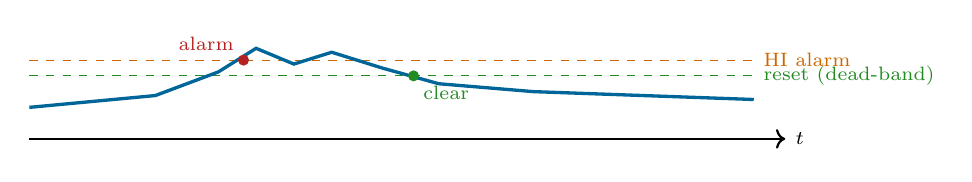
\begin{tikzpicture}[font=\scriptsize, x=0.8cm, y=0.5cm]
			\draw[->, thick] (0,0) -- (12,0) node[right] {$t$};
			\draw[dashed, cOrange] (0,2) -- (11.5,2) node[right] {HI alarm};
			\draw[dashed, cGreen] (0,1.6) -- (11.5,1.6) node[right] {reset (dead-band)};
			\draw[very thick, cAccent] (0,0.8) -- (2,1.1) -- (3,1.7) -- (3.6,2.3) -- (4.2,1.9) -- (4.8,2.2) -- (5.6,1.8) -- (6.5,1.4) -- (8,1.2) -- (11.5,1.0);
			\fill[cRed] (3.4,2) circle (2pt) node[above left] {alarm};
			\fill[cGreen] (6.1,1.6) circle (2pt) node[below right] {clear};
		\end{tikzpicture}
	\end{frame}

	% =================================================================
	\section{Control of Discrete Manufacturing Processes}
	% =================================================================
	\begin{frame}{Continuous vs.\ Discrete Control}
		\renewcommand{\arraystretch}{1.3}
		\centering
		\small
		\begin{tabular}{@{}>{\raggedright}p{3.0cm}>{\raggedright}p{4.6cm}>{\raggedright\arraybackslash}p{4.6cm}@{}}
			\toprule
			\textbf{Aspect} & \textbf{Continuous control} & \textbf{Discrete control} \\
			\midrule
			Variables   & analog (temperature, flow)     & binary (part present, valve open) \\
			Changes     & continuously in time           & at \textbf{events} (switch closes, timer ends) \\
			Model       & differential equations         & Boolean logic, state machines \\
			Controller  & PID, feedforward               & logic \& sequence control (PLC) \\
			Example     & jacket-water temperature       & conveyor, pick-and-place, batch steps \\
			\bottomrule
		\end{tabular}
		\vspace{0.3cm}
		\begin{block}{Two kinds of discrete control}
			\small \textbf{Logic control} --- outputs depend only on \emph{present} inputs (combinational, interlocks).\\
			\textbf{Sequence control} --- outputs depend on the \emph{step} the process is in (sequential, memory).
		\end{block}
	\end{frame}

	\begin{frame}{Logic Control and Interlocks}
		\begin{columns}[T]
			\begin{column}{0.5\textwidth}
				\begin{block}{Example: press safety interlock}
					\small The press may close only if \textbf{both} hands are on the buttons (L, R), the guard G is closed, and there is no emergency stop E:
					\[
					\text{PRESS} = L \cdot R \cdot G \cdot \overline{E}
					\]
				\end{block}
				\begin{itemize}\small
					\item Interlocks prevent unsafe \textbf{combinations}.
					\item Permissives allow a start only when conditions are met.
				\end{itemize}
			\end{column}
			\begin{column}{0.5\textwidth}
				\renewcommand{\arraystretch}{1.1}
				\centering
				\small
				\begin{tabular}{@{}ccccc@{}}
					\toprule
					$L$ & $R$ & $G$ & $E$ & \textbf{PRESS} \\
					\midrule
					1 & 1 & 1 & 0 & \textbf{1} \\
					1 & 1 & 1 & 1 & 0 \\
					1 & 1 & 0 & 0 & 0 \\
					1 & 0 & 1 & 0 & 0 \\
					0 & 1 & 1 & 0 & 0 \\
					\bottomrule
				\end{tabular}
				\vspace{0.2cm}

				\footnotesize Only one row of the 16 combinations lets the press close.
			\end{column}
		\end{columns}
	\end{frame}

	\begin{frame}{Sequence Control with SFC (Grafcet)}
		\begin{columns}[T]
			\begin{column}{0.45\textwidth}
				\centering
				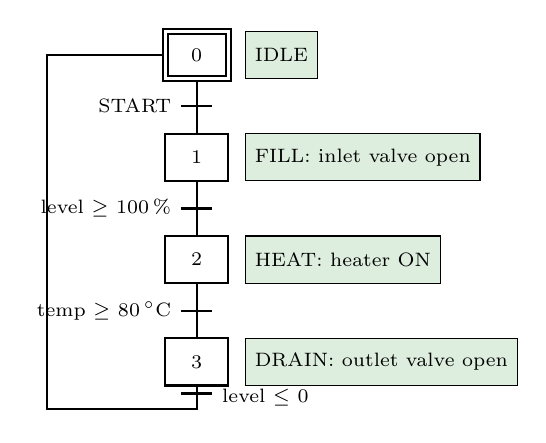
\begin{tikzpicture}[font=\scriptsize,
					sfcstep/.style={rectangle, draw, thick, minimum width=0.8cm, minimum height=0.6cm},
					act/.style={rectangle, draw, fill=cGreen!15, minimum height=0.6cm, align=left}]
					\node[sfcstep, double, double distance=1pt] (s0) at (0,0) {0};
					\node[act, right=0.2cm of s0] {IDLE};
					\node[sfcstep] (s1) at (0,-1.3) {1};
					\node[act, right=0.2cm of s1] {FILL: inlet valve open};
					\node[sfcstep] (s2) at (0,-2.6) {2};
					\node[act, right=0.2cm of s2] {HEAT: heater ON};
					\node[sfcstep] (s3) at (0,-3.9) {3};
					\node[act, right=0.2cm of s3] {DRAIN: outlet valve open};
					\foreach \a/\b/\t in {s0/s1/START, s1/s2/{level $\ge$ 100\,\%}, s2/s3/{temp $\ge$ 80\,$^\circ$C}} {
						\draw[thick] (\a) -- (\b);
						\draw[thick] ($(\a)!0.5!(\b)+(-0.2,0)$) -- ($(\a)!0.5!(\b)+(0.2,0)$);
						\node[left] at ($(\a)!0.5!(\b)+(-0.2,0)$) {\t};
					}
					\draw[thick] (s3) -- ++(0,-0.6) coordinate (b) -- ++(-1.9,0) |- (s0.west);
					\draw[thick] ($(s3)+(-0.2,-0.4)$) -- ($(s3)+(0.2,-0.4)$);
					\node[right] at ($(s3)+(0.2,-0.45)$) {level $\le$ 0};
				\end{tikzpicture}
			\end{column}
			\begin{column}{0.55\textwidth}
				\begin{itemize}\small
					\item \textbf{Steps} (boxes) --- the state the process is in; the active step's \textbf{actions} are ON.
					\item \textbf{Transitions} (bars) --- conditions that move to the next step.
					\item Double box = \textbf{initial step}.
					\item SFC supports branches: alternative (OR) and simultaneous (AND) sequences.
				\end{itemize}
				\begin{block}{Same thing in software}
					\small An SFC is a \textbf{state machine}: a variable holds the current step, and each scan checks only the transition out of that step. The C program on the next slide does exactly this.
				\end{block}
			\end{column}
		\end{columns}
	\end{frame}

	\begin{frame}[fragile, plain]{}

		\vspace*{0.05cm}

		\begin{columns}[T,onlytextwidth]

			% =========================================================
			% LEFT COLUMN -- PSEUDOCODE
			% =========================================================

			\begin{column}{0.21\textwidth}

				\begin{block}{Pseudocode}
					\scriptsize
					\begin{enumerate}
						\item START in state FILL
						\item \textbf{REPEAT} each scan until DONE
						\begin{itemize}\scriptsize
							\item FILL: level += 20; if level $\ge$ 100 $\to$ HEAT
							\item HEAT: temp += 15; if temp $\ge$ 80 $\to$ DRAIN
							\item DRAIN: level $-$= 25; if level $\le$ 0 $\to$ DONE
							\item PRINT state, level, temp
						\end{itemize}
						\item STOP
					\end{enumerate}
				\end{block}

			\end{column}


			% =========================================================
			% MIDDLE COLUMN -- C PROGRAM
			% =========================================================
			\hspace*{0.3cm}
			\begin{column}{0.53\textwidth}

				\begin{block}{C Program (tank state machine)}

\begin{lstlisting}[style=cstyle,numbers=none,basicstyle=\ttfamily\scriptsize]
#include <stdio.h>
enum state { FILL, HEAT, DRAIN, DONE };

int main(void)
{
	const char *name[] = {"FILL","HEAT","DRAIN","DONE"};
	enum state s = FILL;
	int level = 0, temp = 20, t = 0;

	while (s != DONE) {
		t++;
		if (s == FILL) {                     /* inlet  */
			level += 20;  if (level >= 100) s = HEAT;
		} else if (s == HEAT) {              /* heater */
			temp += 15;   if (temp >= 80)   s = DRAIN;
		} else if (s == DRAIN) {             /* outlet */
			level -= 25;  if (level <= 0)   s = DONE;
		}
		printf("t=%2d %-5s L=%3d T=%d\n",
		       t, name[s], level, temp);
	}
	return 0;
}
\end{lstlisting}

				\end{block}

			\end{column}


			% =========================================================
			% RIGHT COLUMN -- OUTPUT
			% =========================================================

			\begin{column}{0.25\textwidth}

				\begin{tikzpicture}[remember picture,overlay]
					\node[
					anchor=north east,
					draw,
					rounded corners=2pt,
					fill=white,
					text width=3.3cm,
					align=left,
					inner sep=6pt
					] at ([xshift=-2mm,yshift=-6mm]current page.north east)
					{
						\textbf{Program Output}\\[3pt]
						\ttfamily\scriptsize
						t= 1 FILL  L= 20 T=20\\
						t= 2 FILL  L= 40 T=20\\
						t= 3 FILL  L= 60 T=20\\
						t= 4 FILL  L= 80 T=20\\
						t= 5 HEAT  L=100 T=20\\
						t= 6 HEAT  L=100 T=35\\
						t= 7 HEAT  L=100 T=50\\
						t= 8 HEAT  L=100 T=65\\
						t= 9 DRAIN L=100 T=80\\
						t=10 DRAIN L= 75 T=80\\
						t=11 DRAIN L= 50 T=80\\
						t=12 DRAIN L= 25 T=80\\
						t=13 DONE  L=  0 T=80
					};
				\end{tikzpicture}

			\end{column}

		\end{columns}

	\end{frame}

	% =================================================================
	\section{Intelligent Systems for Monitoring, Supervision and Control}
	% =================================================================
	\begin{frame}{Intelligent Systems in Industrial Control}
		\begin{columns}[T]
			\begin{column}{0.5\textwidth}
				\begin{block}{Why ``intelligent''?}
					\small Classical controllers need an accurate model and fixed rules. Intelligent techniques use \textbf{expert knowledge}, \textbf{data} and \textbf{learning} to handle complex, uncertain or changing processes.
				\end{block}
				\begin{itemize}\small
					\item \textbf{Expert systems} --- IF--THEN rules from experienced operators.
					\item \textbf{Fuzzy logic} --- control with vague terms (``slightly hot'').
					\item \textbf{Neural networks / ML} --- learn patterns from data.
				\end{itemize}
			\end{column}
			\begin{column}{0.5\textwidth}
				\renewcommand{\arraystretch}{1.25}
				\centering
				\small
				\begin{tabular}{@{}>{\raggedright}p{2.1cm}>{\raggedright\arraybackslash}p{3.6cm}@{}}
					\toprule
					\textbf{Task} & \textbf{Intelligent technique} \\
					\midrule
					Monitoring   & soft sensors, anomaly detection \\
					Supervision  & expert systems, fault diagnosis \\
					Control      & fuzzy control, adaptive / MPC \\
					Maintenance  & predictive maintenance (ML) \\
					Optimisation & genetic algorithms, digital twins \\
					\bottomrule
				\end{tabular}
			\end{column}
		\end{columns}
	\end{frame}

	\begin{frame}{Expert Systems for Supervision}
		\begin{columns}[T]
			\begin{column}{0.5\textwidth}
				\centering
				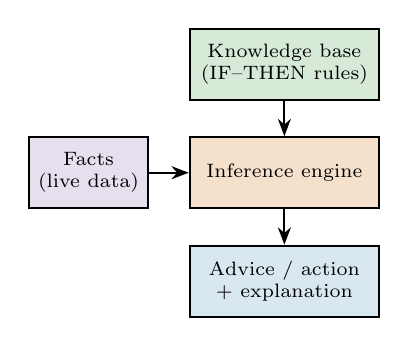
\begin{tikzpicture}[font=\scriptsize, node distance=0.45cm]
					\node[blk, fill=cGreen!18, minimum width=2.4cm] (kb) {Knowledge base\\ (IF--THEN rules)};
					\node[blk, below=of kb, fill=cOrange!20, minimum width=2.4cm] (ie) {Inference engine};
					\node[blk, left=0.5cm of ie, fill=cPurple!15, minimum width=1.4cm] (fd) {Facts\\ (live data)};
					\node[blk, below=of ie, fill=cAccent!15, minimum width=2.4cm] (ui) {Advice / action\\ + explanation};
					\draw[sig] (kb) -- (ie); \draw[sig] (fd) -- (ie); \draw[sig] (ie) -- (ui);
				\end{tikzpicture}
			\end{column}
			\begin{column}{0.5\textwidth}
				\begin{block}{Example rules (engine-room pump)}
					\small
					IF discharge pressure LOW \textbf{AND} motor current LOW\\
					\quad THEN suspect \textbf{loss of suction}.\\[3pt]
					IF discharge pressure LOW \textbf{AND} motor current HIGH\\
					\quad THEN suspect \textbf{blocked impeller / bearing}.\\[3pt]
					IF bearing temp RISING \textbf{AND} vibration HIGH\\
					\quad THEN advise \textbf{stop \& inspect}.
				\end{block}
				\footnotesize Rules capture the experience of senior engineers and \emph{explain} their conclusions.
			\end{column}
		\end{columns}
	\end{frame}

	\begin{frame}{Fuzzy Logic Control: Worked Example}
		\begin{columns}[T]
			\begin{column}{0.5\textwidth}
				\begin{block}{Idea}
					\small Inputs belong to sets like SMALL or LARGE with a \textbf{degree} $\mu$ between 0 and 1; rules fire partially; outputs are blended.
				\end{block}
				\centering
				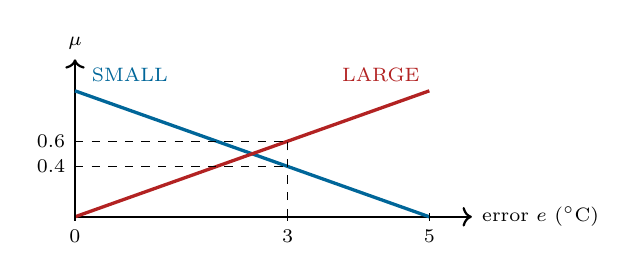
\begin{tikzpicture}[font=\scriptsize, x=0.9cm, y=1.6cm]
					\draw[->, thick] (0,0) -- (5.6,0) node[right] {error $e$ ($^\circ$C)};
					\draw[->, thick] (0,0) -- (0,1.25) node[above] {$\mu$};
					\draw[very thick, cAccent] (0,1) -- (5,0);
					\draw[very thick, cRed] (0,0) -- (5,1);
					\node[cAccent, above right] at (0.1,1) {SMALL};
					\node[cRed, above left] at (5,1) {LARGE};
					\draw[dashed] (3,0) -- (3,0.6);
					\draw[dashed] (0,0.6) -- (3,0.6) node[pos=0, left] {0.6};
					\draw[dashed] (0,0.4) -- (3,0.4) node[pos=0, left] {0.4};
					\foreach \x in {0,3,5} \draw (\x,0.03) -- (\x,-0.03) node[below] {\x};
				\end{tikzpicture}
			\end{column}
			\begin{column}{0.5\textwidth}
				\textbf{Rules:}\\
				\small IF $e$ is SMALL THEN heater $= 20\,\%$\\
				IF $e$ is LARGE THEN heater $= 80\,\%$
				\vspace{0.15cm}

				\textbf{Input} $e = 3\,^\circ$C:\quad $\mu_S = 0.4$, \; $\mu_L = 0.6$
				\vspace{0.1cm}

				\textbf{Weighted average (Sugeno):}
				\[
				u = \frac{0.4\times20 + 0.6\times80}{0.4 + 0.6} = \boxed{56\,\%}
				\]
				\footnotesize Smooth output from simple rules --- used in washing machines, cement kilns, ship stabilisers and autopilots.
			\end{column}
		\end{columns}
	\end{frame}

	\begin{frame}{Condition Monitoring and Predictive Maintenance}
		\begin{columns}[T]
			\begin{column}{0.5\textwidth}
				\begin{itemize}\small
					\item Measure health indicators: \textbf{vibration}, temperature, oil debris, current signature, pressure drop.
					\item Detect \textbf{trends} early and plan repair before failure.
					\item ML models learn the ``normal'' behaviour and flag \textbf{anomalies}.
					\item Estimate \textbf{remaining useful life (RUL)}.
				\end{itemize}
				\begin{block}{Maintenance strategies}
					\small Breakdown $\rightarrow$ preventive (by calendar) $\rightarrow$ \textbf{predictive} (by condition).
				\end{block}
			\end{column}
			\begin{column}{0.5\textwidth}
				\centering
				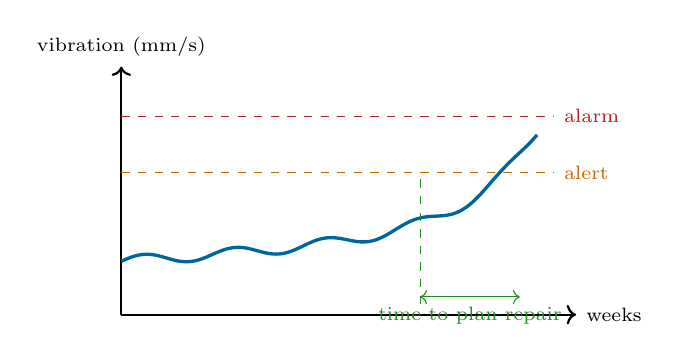
\begin{tikzpicture}[font=\scriptsize, x=0.55cm, y=0.45cm]
					\draw[->, thick] (0,0) -- (10.5,0) node[right] {weeks};
					\draw[->, thick] (0,0) -- (0,7) node[above] {vibration (mm/s)};
					\draw[dashed, cOrange] (0,4) -- (10,4) node[right] {alert};
					\draw[dashed, cRed] (0,5.6) -- (10,5.6) node[right] {alarm};
					\draw[very thick, cAccent, domain=0:9.6, samples=60, smooth] plot (\x, {1.5 + 0.08*\x + 0.9*exp((\x-9.6)/1.6)*3.2 + 0.15*sin(deg(3*\x))});
					\draw[<->, cGreen] (6.9,0.5) -- (9.2,0.5) node[midway, below] {time to plan repair};
					\draw[dashed, cGreen] (6.9,0.3) -- (6.9,4);
				\end{tikzpicture}
			\end{column}
		\end{columns}
	\end{frame}

	\begin{frame}{Fault Detection and Diagnosis}
		\centering
		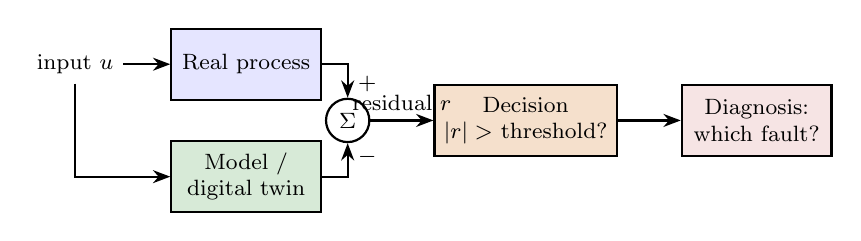
\begin{tikzpicture}[font=\footnotesize, node distance=0.8cm]
			\node (u) {input $u$};
			\node[blk, right=0.6cm of u, fill=blue!10] (p) {Real process};
			\node[blk, below=0.5cm of p, fill=cGreen!18] (m) {Model /\\ digital twin};
			\node[sumj, right=1.0cm of $(p)!0.5!(m)$] (s) {$\Sigma$};
			\node[blk, right=0.8cm of s, fill=cOrange!20] (d) {Decision\\ $|r| > $ threshold?};
			\node[blk, right=0.8cm of d, fill=cRed!12] (dg) {Diagnosis:\\ which fault?};
			\draw[sig] (u) -- (p);
			\draw[sig] (u.south) |- (m);
			\draw[sig] (p.east) -| node[pos=0.8, right] {$+$} (s.north);
			\draw[sig] (m.east) -| node[pos=0.8, right] {$-$} (s.south);
			\draw[sig] (s) -- node[above] {residual $r$} (d);
			\draw[sig] (d) -- (dg);
		\end{tikzpicture}
		\vspace{0.3cm}
		\begin{itemize}\small
			\item \textbf{Residual} = measured output $-$ model output; near zero when healthy.
			\item A residual above the threshold \textbf{detects} a fault; the pattern of residuals \textbf{isolates} it (sensor, actuator or process fault).
			\item Supervisory system then reconfigures: switch to a standby pump, use a backup sensor, or shut down safely.
		\end{itemize}
	\end{frame}

	% =================================================================
	\section{Case Studies of Industrial Control Systems}
	% =================================================================
	\begin{frame}{Case Study 1: Boiler Drum Level --- Three-Element Control}
		\begin{columns}[T]
			\begin{column}{0.5\textwidth}
				\centering
				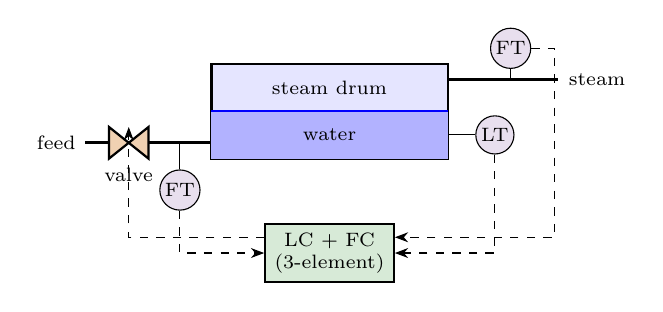
\begin{tikzpicture}[font=\scriptsize]
					% drum
					\draw[thick, fill=blue!10] (0,2) rectangle (3,3.2);
					\fill[blue!30] (0,2) rectangle (3,2.6);
					\draw[blue, thick] (0,2.6) -- (3,2.6);
					\node at (1.5,2.3) {water};
					\node at (1.5,2.9) {steam drum};
					% steam out
					\draw[very thick] (3,3.0) -- (4.4,3.0) node[right] {steam};
					\node[circle, draw, fill=cPurple!15, inner sep=1pt] (ft1) at (3.8,3.4) {FT};
					\draw (ft1) -- (3.8,3.0);
					% feedwater in
					\draw[very thick] (-1.6,2.2) -- (0,2.2);
					\filldraw[fill=cOrange!30, thick] (-1.3,2.0) -- (-1.3,2.4) -- (-0.8,2.0) -- (-0.8,2.4) -- cycle;
					\node[below] at (-1.05,2.0) {valve};
					\node[circle, draw, fill=cPurple!15, inner sep=1pt] (ft2) at (-0.4,1.6) {FT};
					\draw (ft2) -- (-0.4,2.2);
					\node[left] at (-1.6,2.2) {feed};
					% level
					\node[circle, draw, fill=cPurple!15, inner sep=1pt] (lt) at (3.6,2.3) {LT};
					\draw (lt) -- (3,2.3);
					% controller
					\node[rectangle, draw, thick, fill=cGreen!18, align=center] (lc) at (1.5,0.8) {LC + FC\\ (3-element)};
					\draw[dashed, -{Stealth}] (lt) |- (lc.east);
					\draw[dashed, -{Stealth}] (ft1.east) -- ++(0.3,0) |- ($(lc.east)+(0,0.2)$);
					\draw[dashed, -{Stealth}] (ft2) |- (lc.west);
					\draw[dashed, -{Stealth}] (lc.west) ++(0,0.2) -| (-1.05,2.4);
				\end{tikzpicture}
			\end{column}
			\begin{column}{0.5\textwidth}
				\begin{itemize}\small
					\item \textbf{Element 1} --- drum level (LT): the variable to control.
					\item \textbf{Element 2} --- steam flow: \textbf{feedforward} of the load.
					\item \textbf{Element 3} --- feedwater flow: fast \textbf{cascade} inner loop.
				\end{itemize}
				\begin{block}{Why not just level control?}
					\small When steam demand rises, pressure falls and bubbles swell --- level \emph{rises} first (\textbf{swell}). A level-only controller would cut feedwater just when more is needed. Feedforward from steam flow avoids this.
				\end{block}
			\end{column}
		\end{columns}
	\end{frame}

	\begin{frame}{Case Study 2: Main Engine Jacket Cooling-Water Temperature}
		\begin{columns}[T]
			\begin{column}{0.5\textwidth}
				\centering
				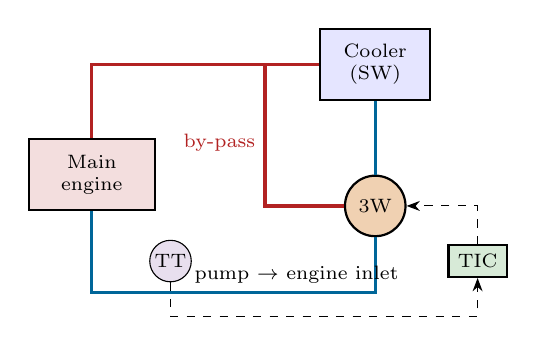
\begin{tikzpicture}[font=\scriptsize]
					\node[blk, fill=cRed!15, minimum width=1.6cm] (eng) at (0,0) {Main\\ engine};
					\node[blk, fill=blue!10, minimum width=1.4cm] (cool) at (3.6,1.4) {Cooler\\ (SW)};
					\node[circle, draw, thick, fill=cOrange!30, minimum size=0.6cm] (v) at (3.6,-0.4) {3W};
					\draw[very thick, cRed] (eng.north) |- (2.2,1.4) -- (cool.west);
					\draw[very thick, cRed] (2.2,1.4) -- (2.2,-0.4) -- (v.west);
					\node[left, cRed] at (2.2,0.4) {by-pass};
					\draw[very thick, cAccent] (cool.south) -- (v.north);
					\draw[very thick, cAccent] (v.south) |- (0,-1.5) -- (eng.south);
					\node[above] at (2.6,-1.5) {pump $\rightarrow$ engine inlet};
					\node[circle, draw, fill=cPurple!15, inner sep=1pt] (tt) at (1.0,-1.1) {TT};
					\node[rectangle, draw, thick, fill=cGreen!18] (tc) at (4.9,-1.1) {TIC};
					\draw[dashed, -{Stealth}] (tt) -- ++(0,-0.7) -| (tc.south);
					\draw[dashed, -{Stealth}] (tc.north) |- (v.east);
				\end{tikzpicture}
			\end{column}
			\begin{column}{0.5\textwidth}
				\begin{itemize}\small
					\item A \textbf{three-way valve} mixes cooled and by-passed water.
					\item \textbf{PID} (TIC) keeps the engine inlet temperature near its setpoint (typically about 80\,$^\circ$C).
					\item Often \textbf{cascade} with outlet temperature, or \textbf{feedforward} from engine load.
					\item Alarms: high temperature, low pressure $\rightarrow$ slow-down / shut-down of the engine (safety system, separate from control).
				\end{itemize}
			\end{column}
		\end{columns}
	\end{frame}

	\begin{frame}{Case Study 3: Bottle-Filling Line (PLC + SCADA)}
		\centering
		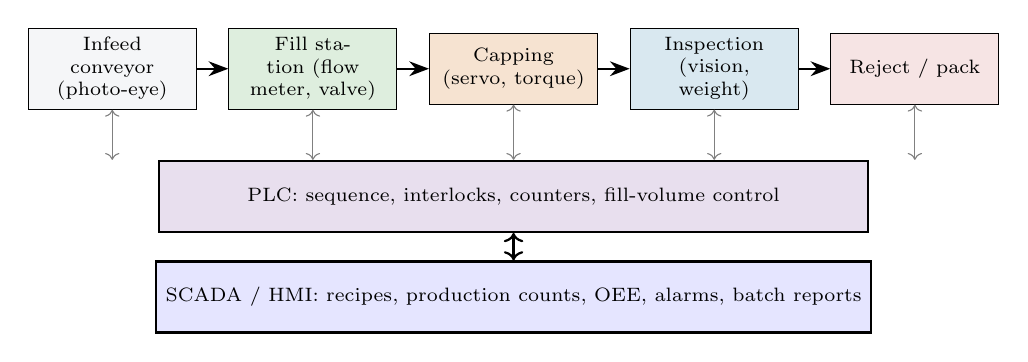
\begin{tikzpicture}[every node/.style={font=\scriptsize}, node distance=0.4cm,
			st/.style={process, minimum width=1.9cm, text width=1.9cm, minimum height=0.9cm}]
			\node[st, fill=cGrayBg] (a) {Infeed conveyor (photo-eye)};
			\node[st, right=of a, fill=cGreen!15] (b) {Fill station (flow meter, valve)};
			\node[st, right=of b, fill=cOrange!18] (c) {Capping (servo, torque)};
			\node[st, right=of c, fill=cAccent!15] (d) {Inspection (vision, weight)};
			\node[st, right=of d, fill=cRed!12] (e) {Reject / pack};
			\draw[flowarrow] (a) -- (b); \draw[flowarrow] (b) -- (c); \draw[flowarrow] (c) -- (d); \draw[flowarrow] (d) -- (e);
			\node[blk, fill=cPurple!15, minimum width=9cm, below=0.7cm of c] (plc) {PLC: sequence, interlocks, counters, fill-volume control};
			\node[blk, fill=blue!10, minimum width=9cm, below=0.35cm of plc] (sc) {SCADA / HMI: recipes, production counts, OEE, alarms, batch reports};
			\foreach \n in {a,b,c,d,e} \draw[<->, gray] (\n.south) -- (\n.south |- plc.north);
			\draw[<->, thick] (plc) -- (sc);
		\end{tikzpicture}
		\vspace{0.2cm}
		\begin{itemize}\small
			\item \textbf{Discrete control}: photo-eyes and counters trigger each station; a state machine per station.
			\item \textbf{Continuous control}: fill flow and capping torque; \textbf{intelligent} vision inspection rejects bad bottles.
			\item SCADA computes \textbf{OEE} = availability $\times$ performance $\times$ quality, e.g.\ $0.90\times0.95\times0.98 = 0.84$.
		\end{itemize}
	\end{frame}

	\begin{frame}{Case Study 4: Ship Alarm, Monitoring and Control System}
		\begin{columns}[T]
			\begin{column}{0.55\textwidth}
				\centering
				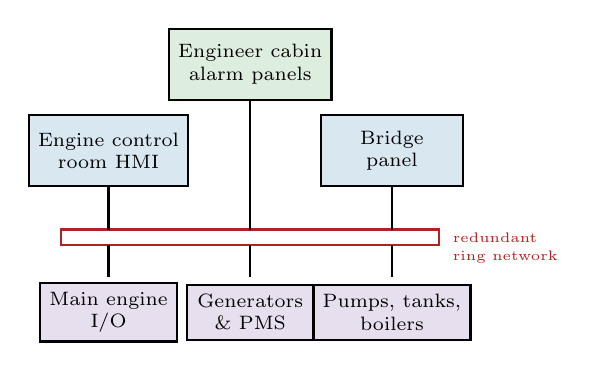
\begin{tikzpicture}[font=\scriptsize]
					\node[blk, fill=cAccent!15, minimum width=1.8cm] (ecr) at (0,2.4) {Engine control\\ room HMI};
					\node[blk, fill=cAccent!15, minimum width=1.8cm] (br) at (3.6,2.4) {Bridge\\ panel};
					\node[blk, fill=cGreen!15, minimum width=1.8cm] (cab) at (1.8,3.5) {Engineer cabin\\ alarm panels};
					\draw[thick, cRed] (-0.6,1.4) -- (4.2,1.4) -- (4.2,1.2) -- (-0.6,1.2) -- cycle;
					\node[font=\tiny, cRed, right] at (4.25,1.3) {redundant};
					\node[font=\tiny, cRed, right] at (4.25,1.05) {ring network};
					\draw[thick] (ecr) -- (0,1.4); \draw[thick] (br) -- (3.6,1.4); \draw[thick] (cab.south) -- (1.8,1.4);
					\foreach \x/\n in {0/{Main engine\\ I/O}, 1.8/{Generators\\ \& PMS}, 3.6/{Pumps, tanks,\\ boilers}} {
						\draw[thick] (\x,1.2) -- (\x,0.8);
						\node[blk, fill=cPurple!15, minimum width=1.6cm, minimum height=0.7cm] at (\x,0.35) {\n};
					}
				\end{tikzpicture}
			\end{column}
			\begin{column}{0.45\textwidth}
				\begin{itemize}\small
					\item Thousands of I/O points: temperatures, pressures, levels, running status.
					\item \textbf{Distributed} I/O stations near the machinery; redundant network.
					\item \textbf{UMS} (unmanned machinery space): alarms routed to the duty engineer's cabin at night.
					\item \textbf{PMS} (power management) starts / stops generators automatically.
					\item Class rules require redundancy, self-monitoring and independent safety systems.
				\end{itemize}
			\end{column}
		\end{columns}
	\end{frame}

	\begin{frame}{Summary \& What Comes Next}
		\begin{columns}[T]
			\begin{column}{0.5\textwidth}
				\begin{block}{Concept}
					\begin{itemize}\small
						\item Digital controller implementation: sampling, ADC/DAC, discrete PID, filtering.
						\item Control strategies: feedforward, cascade, ratio, split-range, override.
						\item PLCs: architecture, scan cycle, IEC 61131-3.
						\item Real-time issues, delay, scheduling, signal transmission.
						\item Industrial networks and protocols.
						\item DAQ, SCADA, DCS, alarm management.
						\item Discrete control, SFC, state machines.
						\item Intelligent systems and case studies.
					\end{itemize}
				\end{block}
			\end{column}
			\begin{column}{0.5\textwidth}
				\begin{block}{Practice makes perfect}
					\begin{itemize}\small
						\item Run both C programs; change gains, sample time and thresholds.
						\item Write the tank sequence in ladder logic or ST.
						\item Recalculate the Modbus poll time at 9600 and 115\,200 baud.
						\item Draw the control scheme of a system on board a ship.
					\end{itemize}
				\end{block}
				\begin{block}{Coming up}
					\small Industrial cybersecurity, safety instrumented systems (SIS) and IIoT / Industry 4.0.
				\end{block}
			\end{column}
		\end{columns}
	\end{frame}

	%------------------------------------------------
	\begin{frame}
		\centering
		\Huge Thank You
		\vspace{0.5cm}

		\normalsize Questions?
	\end{frame}

	%------------------------------------------------

\end{document}
